%%
%% Author: david
%% 17/04/19
%%

% Preamble
\documentclass[french,a4paper,11pt]{article}

\addtolength{\hoffset}{-3cm}
\addtolength{\textwidth}{6cm}

\usepackage{minted}
\usepackage{babel}
\usepackage[utf8]{inputenc}
\usepackage{amsmath}
\usepackage{amsfonts}
\usepackage{xcolor,graphicx}
\usepackage{float}
\usepackage{fancyhdr}
\usepackage{subfig}
\usepackage{url}
\usepackage[T1]{fontenc}

\captionsetup[subfigure]{labelformat=empty}

\setlength{\parindent}{0pt}

\title{Labo 1 Advanced Cloud\\APP SCALING ON AMAZON WEB SERVICES}

\author{David Wittwer \and Ludovic Gindre}

\begin{document}
    \maketitle
    \section{Introduction}\label{sec:introduction}
    Voici le compte rendu tu TP "APP SCALING ON AMAZON WEB SERVICES" que nous avons réalisé

    \section{Tache 2}\label{sec:task-2}

    \begin{figure}
        \center{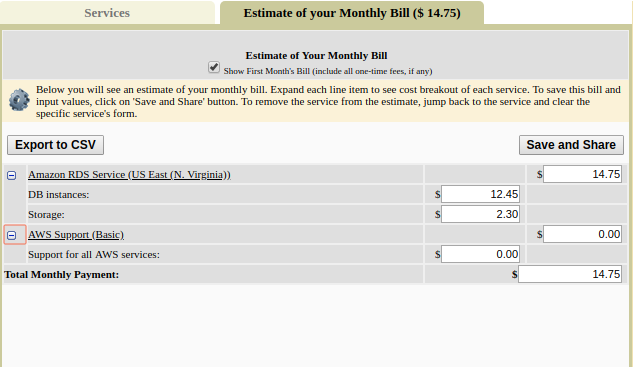
\includegraphics[width=\textwidth]{assets/drupal_db_cost.png}}
        \caption{\label{rds-costs}Coûts instance RDS}
    \end{figure}
    Comme on peux le voir sur la figure \ref{rds-costs}, Le coût mensuel d'une instance RDS de classe db.t2.micro est de 17.75\$

    \section{Tache 4}\label{sec:task-4}

    \begin{figure}
        \center{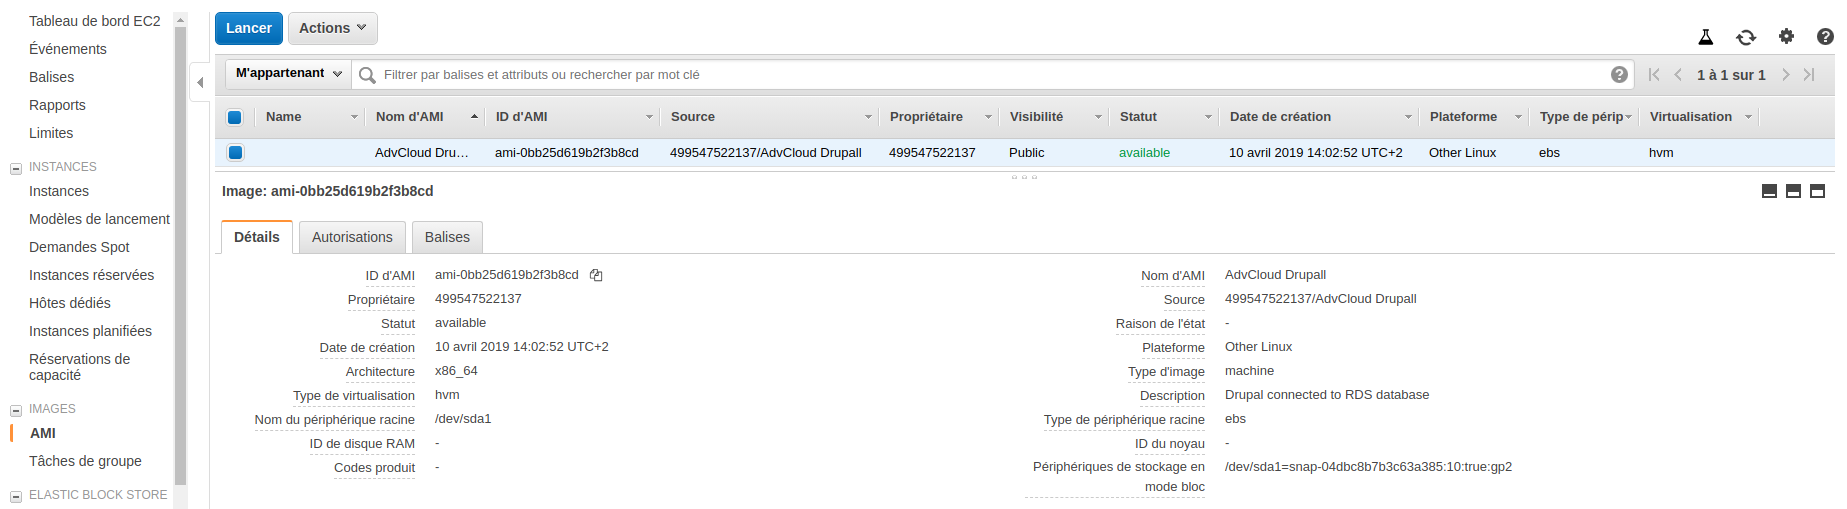
\includegraphics[width=\textwidth]{assets/ami.png}}
        \caption{\label{ami-details}Détail de l'image crée}
    \end{figure}

    La figure \ref{ami-details} nous montre les détails de l'AMI crée.
    Le cout d'une AMI dépend du cout du snashot de l'instance EC2.
    Dans notre cas, un disque de 10 Go était sur l'instance donc cela nous fait un snapshot de 10 Go ce qui selon le calculateur AWS coute 0.50\$ par mois

    \section{Tache 5}\label{sec:task-5}

    \begin{figure}
        \center{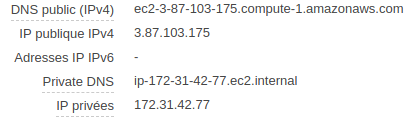
\includegraphics[width=\textwidth]{assets/instance_ip.png}}
        \caption{\label{ec2-ip}Adresse IP de l'instance EC2}
    \end{figure}

    \begin{figure}
        \center{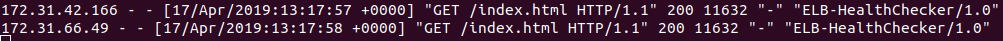
\includegraphics[width=\textwidth]{assets/load_balancer_ips.png}}
        \caption{\label{lb-ip}Adresse ip du load balancer depuis l'instance}
    \end{figure}

    \begin{figure}
        \center{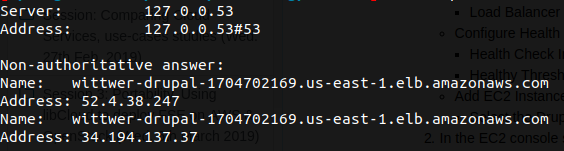
\includegraphics[width=\textwidth]{assets/nslookup_lb.png}}
        \caption{\label{dns-ip}Adresse ip du load balancer avec nslookup}
    \end{figure}

    Sur la figure \ref{ec2-ip}, on peux voir que l'adresse IP publique de l'instance EC2 est: 3.87.103.175 or, lors du
    dnslookup que l'on peux voir sur la figure \ref{dns-ip} on obtient deux adresses IP mais que aucune n'est celle de l'instance.
    Ceci est du au fait que le load balancer n'expose pas les adresses IP de l'instance pour pouvoir rediriger vers l'instance qu'il a choisi.
    De plus, cela permet aussi que si un instance vient à être indisponible, le load balancer redirigera vers une autre de maniètre tranparente pour l'utilisateur.

    Su la figure \ref{lb-ip}, on peux voir que les adresses IP pour la vérification de sante de l'instance sont des adresse de réseau interne de AWS.

    \section{Tache 6}\label{sec:task-6}

    \begin{figure}
        \center{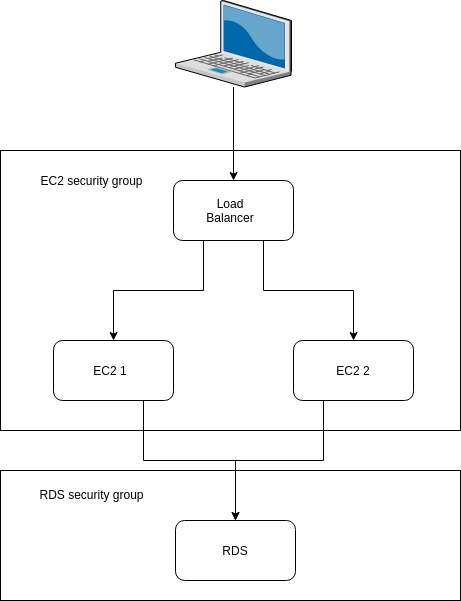
\includegraphics[width=\textwidth]{assets/architecture.png}}
        \caption{\label{archi}Architecture globale du labo}
    \end{figure}

    \begin{figure}
        \center{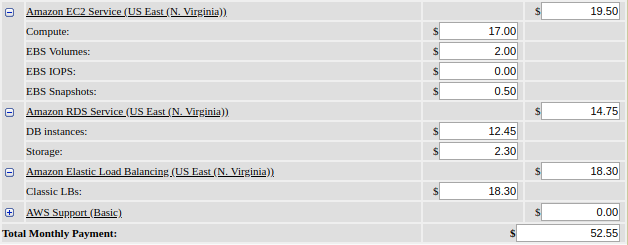
\includegraphics[width=\textwidth]{assets/total_cost.png}}
        \caption{\label{total-cost}Cout total mensuel du labo}
    \end{figure}

    \begin{figure}
        \center{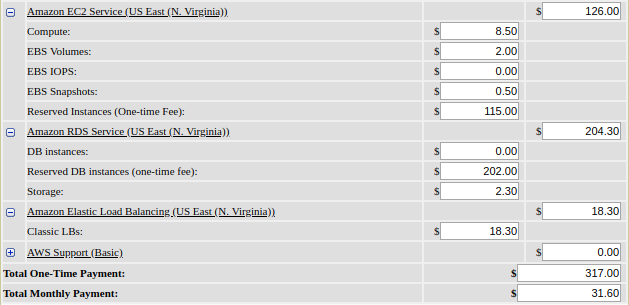
\includegraphics[width=\textwidth]{assets/total_reserved_cost.png}}
        \caption{\label{total-cost-reserved}Cout total mensuel du labo avec 1 EC2 et 1 RDS réservée}
    \end{figure}

    Sur la figure \ref{archi} on peux voir l'architecture globale avec le load balancer, les instance et la base de donnée.
    Le cout mensuel de cette architecture est de 52.55\$.
    Ce cout peux être considérablement diminué si on prend une instance EC2 réservée et l'instance RDS réservée comme on peux le voir sur la figure \ref{total-cost-reserved}.
    Si on divise le cous d'achat des instance par 36 mois cela nous fait un cout mensuel de 8.81\$ soit un cout total mensuel de 40.41\$ par mois.




\end{document}
